% Rotaciones SO(3) en 3D
% Compilar con: pdflatex so3_rotations.tex
\documentclass[tikz,border=10pt]{standalone}
\usepackage{tikz}
\usepackage{amsmath,amssymb}
\usetikzlibrary{arrows.meta, 3d, calc}

\definecolor{gdlblue}{RGB}{41, 98, 168}
\definecolor{gdlred}{RGB}{191, 49, 49}
\definecolor{gdlgreen}{RGB}{30, 130, 76}
\definecolor{gdlorange}{RGB}{217, 130, 30}
\definecolor{gdlpurple}{RGB}{118, 56, 138}
\definecolor{gdlgray}{RGB}{140, 140, 140}
\definecolor{gdlyellow}{RGB}{190, 140, 10}

\begin{document}
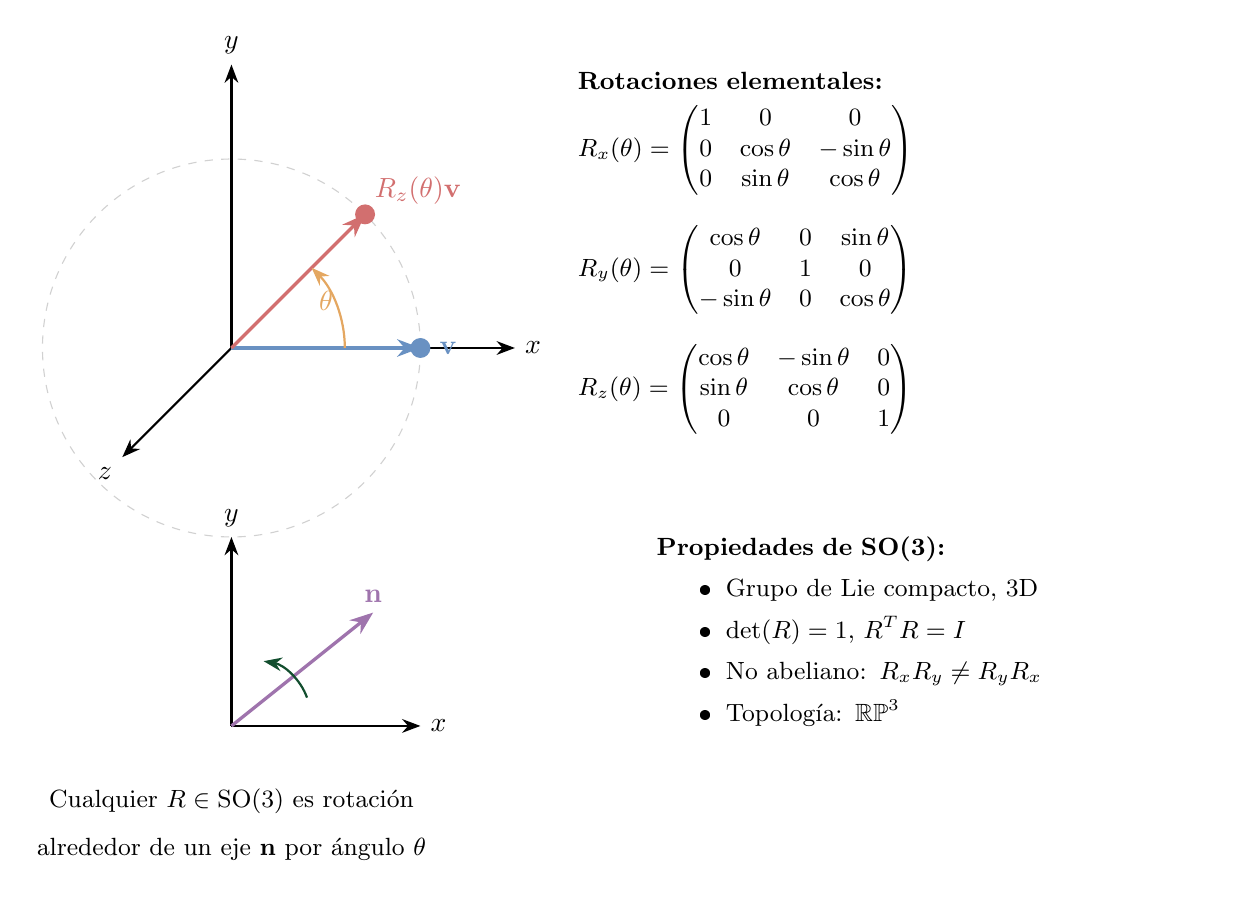
\begin{tikzpicture}[>=Stealth, scale=1.2]

% === Ejes coordenados ===
\draw[thick, ->] (0,0,0) -- (3,0,0) node[right] {$x$};
\draw[thick, ->] (0,0,0) -- (0,3,0) node[above] {$y$};
\draw[thick, ->] (0,0,0) -- (0,0,3) node[below left] {$z$};

% === Esfera unitaria (sugerida) ===
\draw[gdlgray!40, dashed] (0,0) circle (2cm);

% === Rotación alrededor de z ===
\begin{scope}[shift={(0,0)}]
    % Vector inicial
    \draw[->, very thick, gdlblue!70] (0,0,0) -- (2,0,0);
    \fill[gdlblue!70] (2,0,0) circle (3pt);
    \node[gdlblue!70, right] at (2.1,0,0) {$\mathbf{v}$};

    % Vector rotado
    \draw[->, very thick, gdlred!70] (0,0,0) -- ({2*cos(45)},{2*sin(45)},0);
    \fill[gdlred!70] ({2*cos(45)},{2*sin(45)},0) circle (3pt);
    \node[gdlred!70, above right] at ({2*cos(45)},{2*sin(45)},0) {$R_z(\theta)\mathbf{v}$};

    % Arco de rotación
    \draw[thick, gdlorange!70, ->] (1.2,0,0) arc (0:45:1.2cm);
    \node[gdlorange!70] at (1, 0.5, 0) {$\theta$};
\end{scope}

% === Matrices de rotación ===
\node[font=\small, text width=8cm] at (7, 1) {
    \textbf{Rotaciones elementales:}\\[0.5em]
    $R_x(\theta) = \begin{pmatrix} 1 & 0 & 0 \\ 0 & \cos\theta & -\sin\theta \\ 0 & \sin\theta & \cos\theta \end{pmatrix}$\\[1em]
    $R_y(\theta) = \begin{pmatrix} \cos\theta & 0 & \sin\theta \\ 0 & 1 & 0 \\ -\sin\theta & 0 & \cos\theta \end{pmatrix}$\\[1em]
    $R_z(\theta) = \begin{pmatrix} \cos\theta & -\sin\theta & 0 \\ \sin\theta & \cos\theta & 0 \\ 0 & 0 & 1 \end{pmatrix}$
};

% === Propiedades ===
\node[font=\small, text width=6cm] at (7, -3) {
    \textbf{Propiedades de SO(3):}
    \begin{itemize}
        \item Grupo de Lie compacto, 3D
        \item $\det(R) = 1$, $R^T R = I$
        \item No abeliano: $R_x R_y \neq R_y R_x$
        \item Topología: $\mathbb{RP}^3$
    \end{itemize}
};

% === Eje de rotación general ===
\begin{scope}[shift={(0,-4)}]
    \draw[thick, ->] (0,0) -- (2,0) node[right] {$x$};
    \draw[thick, ->] (0,0) -- (0,2) node[above] {$y$};

    % Eje arbitrario
    \draw[very thick, gdlpurple!70, ->] (0,0) -- (1.5,1.2);
    \node[gdlpurple!70, above] at (1.5,1.2) {$\mathbf{n}$};

    % Rotación alrededor de n
    \draw[thick, gdlgreen!60!black, ->] (0.8,0.3) arc (20:80:0.6cm);

    \node[font=\small] at (0, -0.8) {Cualquier $R \in \mathrm{SO}(3)$ es rotación};
    \node[font=\small] at (0, -1.3) {alrededor de un eje $\mathbf{n}$ por ángulo $\theta$};
\end{scope}

\end{tikzpicture}
\end{document}
